\subsubsection{Morphology}
\label{subsubsection:morphology}
Morphological operators are a set of neighborhood operators that modify the shape of objects in binary images. A binary image is most often produced by thresholding (see section \ref{subsection:thresholding}) a grayscale image, Figure \ref{fig:thresholding} shows the conversion of an RGB image to a binary one, here the white pixels are regarded as objects sometimes referred to as 'blobs'.Morphological operations are used if you wish to modify blobs, for example to change total area of blob and to connect or separate two or more blobs. Morphological operators, like filters, depend on a kernel that characterises their behaviour which is called a \emph{structuring element}. There are two fundamental morphological operations, \emph{dilation} and \emph{erosion}, that all others are a combination of \cite{morph_textbook}. 

\begin{figure}[htbp]
    \centering
    \begin{subfigure}[b]{0.3\textwidth}
        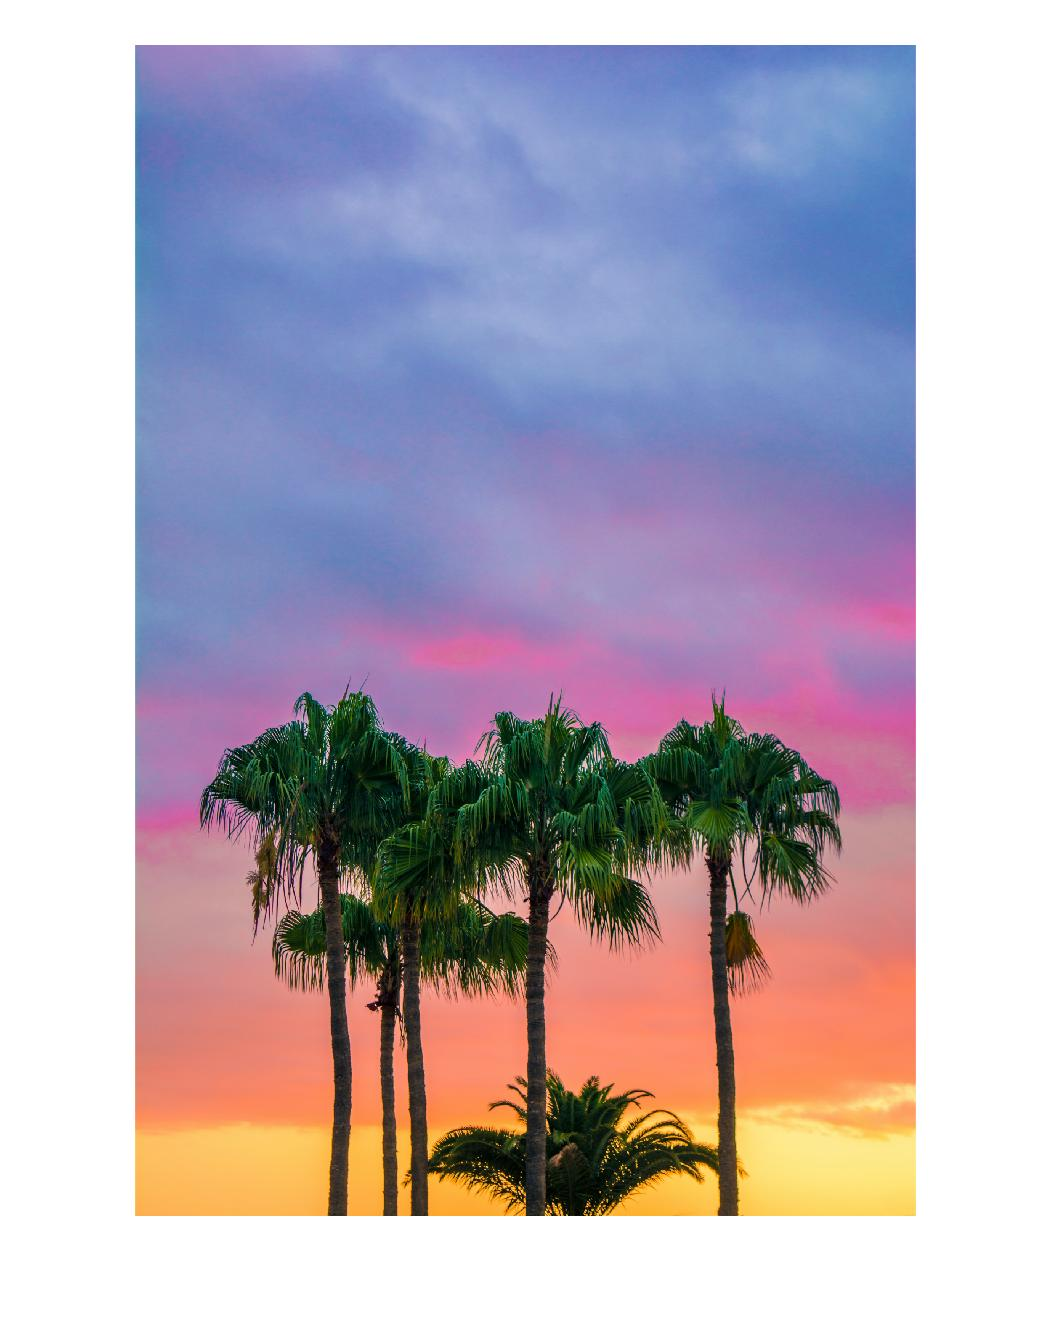
\includegraphics[width=\textwidth]{palms_resized}
        \caption{RGB Image}
        \label{fig:emu_noise}
    \end{subfigure}
    \begin{subfigure}[b]{0.3\textwidth}
        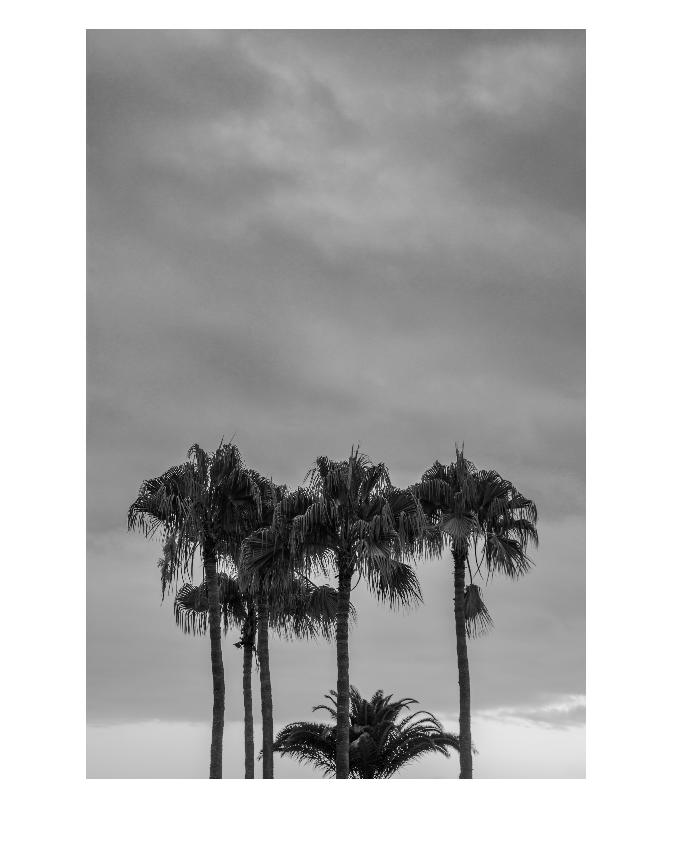
\includegraphics[width=\textwidth]{palms_grayscale}
        \caption{Grayscale Conversion}
        \label{fig:emu_gauss}
    \end{subfigure}
    \begin{subfigure}[b]{0.3\textwidth}
        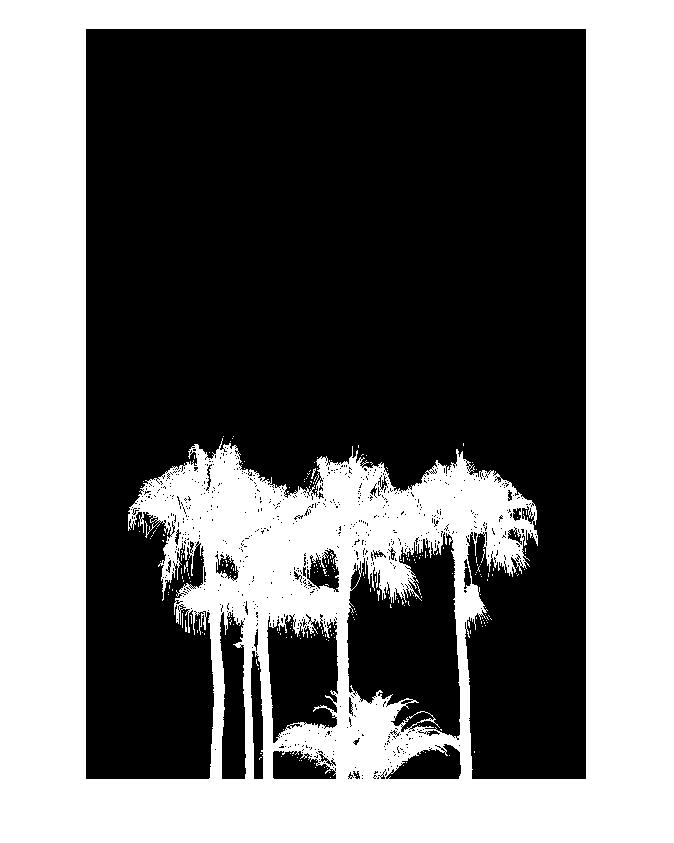
\includegraphics[width=\textwidth]{palms_binary}
        \caption{Binary Thresholding}
        \label{fig:emu_median}
    \end{subfigure}
    \captionsetup{format = hang}
    \caption{Conversion of an RGB image to a binary image. Original image by Adam Birkett}
    \label{fig:thresholding}
\end{figure}

\subsubsection{Structuring Elements}

A 2D structuring element itself is a matrix of binary values, generally a smaller than the image it's to operate on, and is of a similar function to a filter kernel, as it largely characterises the effect of the morphological operation it's being used for. A structuring element has a reference pixel or origin that determines where the result of the morphological operation is stored in the output image. Structuring element shapes are selected according to the scenario it's to be used in, for example if you want to produce round edges on blobs you might use a disc structuring element and if you want to produce straight edges you would use a rectangular structing element. Figure \ref{fig:structuring_elements} shows some example shape and size structuring elements. Structuring elements must always have odd dimensions so as to have a centred origin at which to store the output.

\begin{figure}[htbp]
    \centering
    \begin{subfigure}[b]{0.3\textwidth}
           \[ \begin{bmatrix}
                1 & 1 & 1 & 1 & 1\\
                1 & 1 & 1 & 1 & 1\\
                1 & 1 & 1 & 1 & 1\\
                1 & 1 & 1 & 1 & 1\\
                1 & 1 & 1 & 1 & 1\\
             \end{bmatrix}\]
        \captionsetup{format = hang}
        \caption{5x5 Rectangular Structuring Element}
    \end{subfigure}
    \begin{subfigure}[b]{0.3\textwidth}
        \[\begin{bmatrix}
            0 & 0 & 1 & 0 & 0\\
            0 & 1 & 1 & 1 & 0\\
            1 & 1 & 1 & 1 & 1\\
            0 & 1 & 1 & 1 & 0\\
            0 & 0 & 1 & 0 & 0\\
         \end{bmatrix}\]
        \captionsetup{format = hang}
        \caption{5x5 Diamond Structuring Element}
    \end{subfigure} 
    \begin{subfigure}[b]{0.3\textwidth}
       \[\begin{bmatrix}
            0 & 0 & 1 & 0 & 0\\
            0 & 0 & 1 & 0 & 0\\
            1 & 1 & 1 & 1 & 1\\
            0 & 0 & 1 & 0 & 0\\
            0 & 0 & 1 & 0 & 0\\
         \end{bmatrix}\]
        \captionsetup{format = hang}
        \caption{5x5 Cross Structuring Element}
    \end{subfigure}
    \captionsetup{format = hang}
    \caption{}
    \label{fig:structuring_elements}
\end{figure}


\subsubsection{Performing a morphological operation}

A morphological operation is performed by first convolving a structuring element with a neighbourhood of an image and then thresholding the result. The threshold level determines the type of operation that is performed \cite{alg_apps}. Algorithm \ref{algorithm:morphological_operation} outlines how a morphological operation can be implemented.

\begin{algorithm}
\SetAlgoLined
\KwIn{Binary Image X of size MxN}
\KwOut{Binary Image Y of size MxN}
Initialize: structuring element se, threshold level T\;
\For{i = 0 to M}
{
    \For{j = 0 to N}
    {
        convolutionSum = se $\ast$ neighborhoodCentered(X[i,j])\;
        \eIf{convolutionSum $\geq$ T}{
            Y[i,j] = 1\;
        }{
            Y[i,j] = 0\;
        }
    }
}
\caption{Performing a morphological operation.}
\label{algorithm:morphological_operation}
\end{algorithm}

\subsubsection{Fundamental Morphological Operations}

\textbf{Dilation} inflates the size of a blob, the scale and nature of the inflation is determined by the size and shape of specific structuring element used for the operation. In Figure \ref{fig:ice_dilation} a square structuring element is used to fill gaps between objects and for their size to increase, this can be useful in situations where we want to combine blobs that are close together but have small gaps between them. In \ref{algorithm:morphological_operation} to specify that we want a dilation to be performed the threshold value should be set to 1. This means that if a single cell of the structuring element shape is touching a blob the output of the operation will be a 1, increasing the size of the blob in that neighbourhood. 

\textbf{Erosion} performs the opposite function to dilation by causing objects to contract rather than grow. To specify an erosion operation the threshold value in Algorithm \ref{algorithm:morphological_operation} should be set to the sum of the elements in the structuring element. This means that for the output of an erosion operation to be 1 the entire structuring element has to be inside of a blob, anywhere the structuring element overlaps black background the blob will be eroded. In Figure \ref{fig:ice_erosion} many smaller entities are erased from the image and blob edges are smoothed. Erosion can be used to clean up small noise-like blobs from binary images but will also modify blobs that are not regarded as noise-like, by shrinking them and smoothing their edges.

\textbf{Opening} is a composite operation comprised of an erosion and then dilation, the same or different structuring element may be used for each. The effect of this order of operations is to first clear away small blobs and increase the smoothness of and separation between existing blobs and then to consolidate the the remaining blobs by performing a dilation. This is a useful operation if you want to join together blobs that are close together but not touching but first remove any noise-like blobs so that they don't become enlarged. Figure \ref{ref:ice_open} shows the effect of opening with a square structuring element, notice that the small blobs are cleared away but the remaining objects are thickened and most original blobs separation is preserved. 

\textbf{Closing} is the dual of opening and performs first a dilation and then an erosion. This order of operations is useful if you wish to consolidate blobs into large single entities before performing an erosion that clean them up and remove any remaining blobs. Figure \ref{fig:ice_close} shows how a closing was able to remove small noise-like entities but preserve and join larger blobs.

\renewcommand{\arraystretch}{0.6} % because \baselinestretch is 1.6667
\begin{figure}[H]
    \centering
    \begin{subfigure}[b]{0.49\textwidth}
        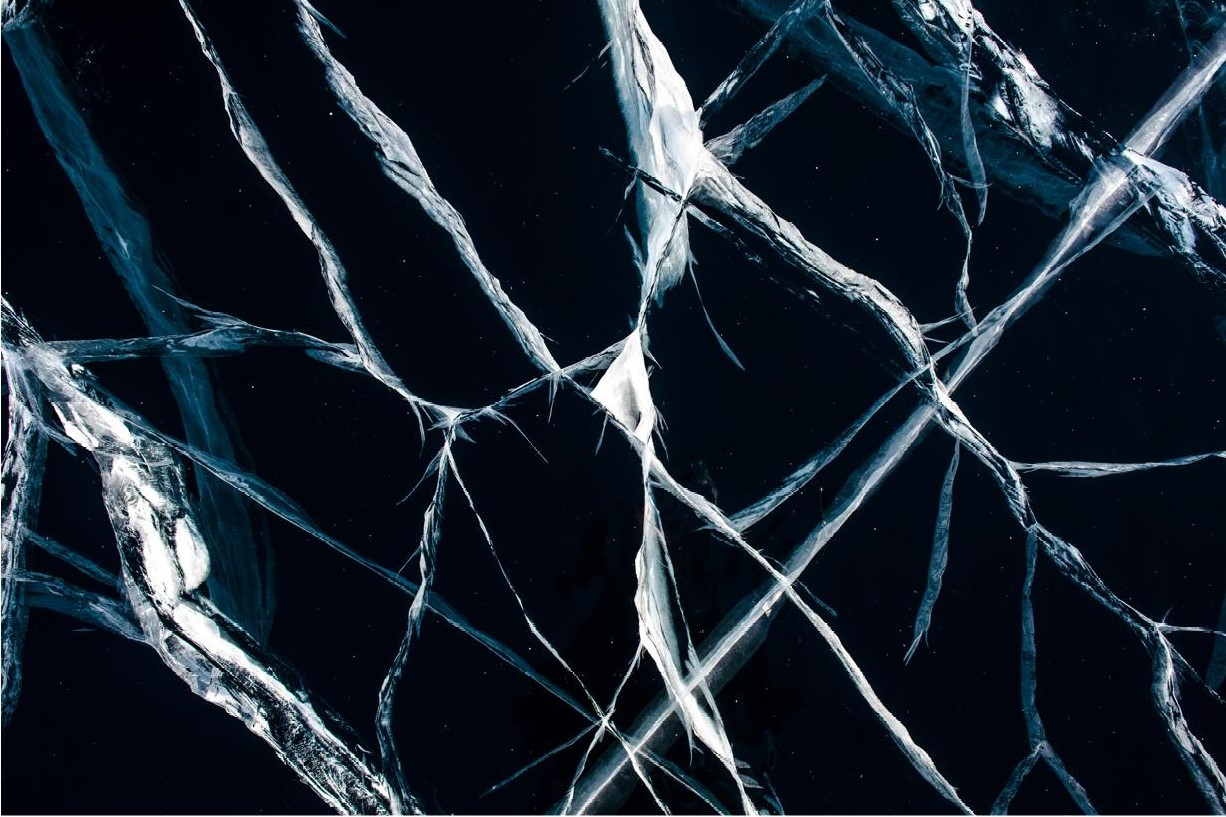
\includegraphics[width=\textwidth]{litreview/imageprocessing/nonlinear/morphology/ice_original}
        \caption{Img: Daniel Born}
        \label{fig:ice}
    \end{subfigure}
    \begin{subfigure}[b]{0.49\textwidth}
        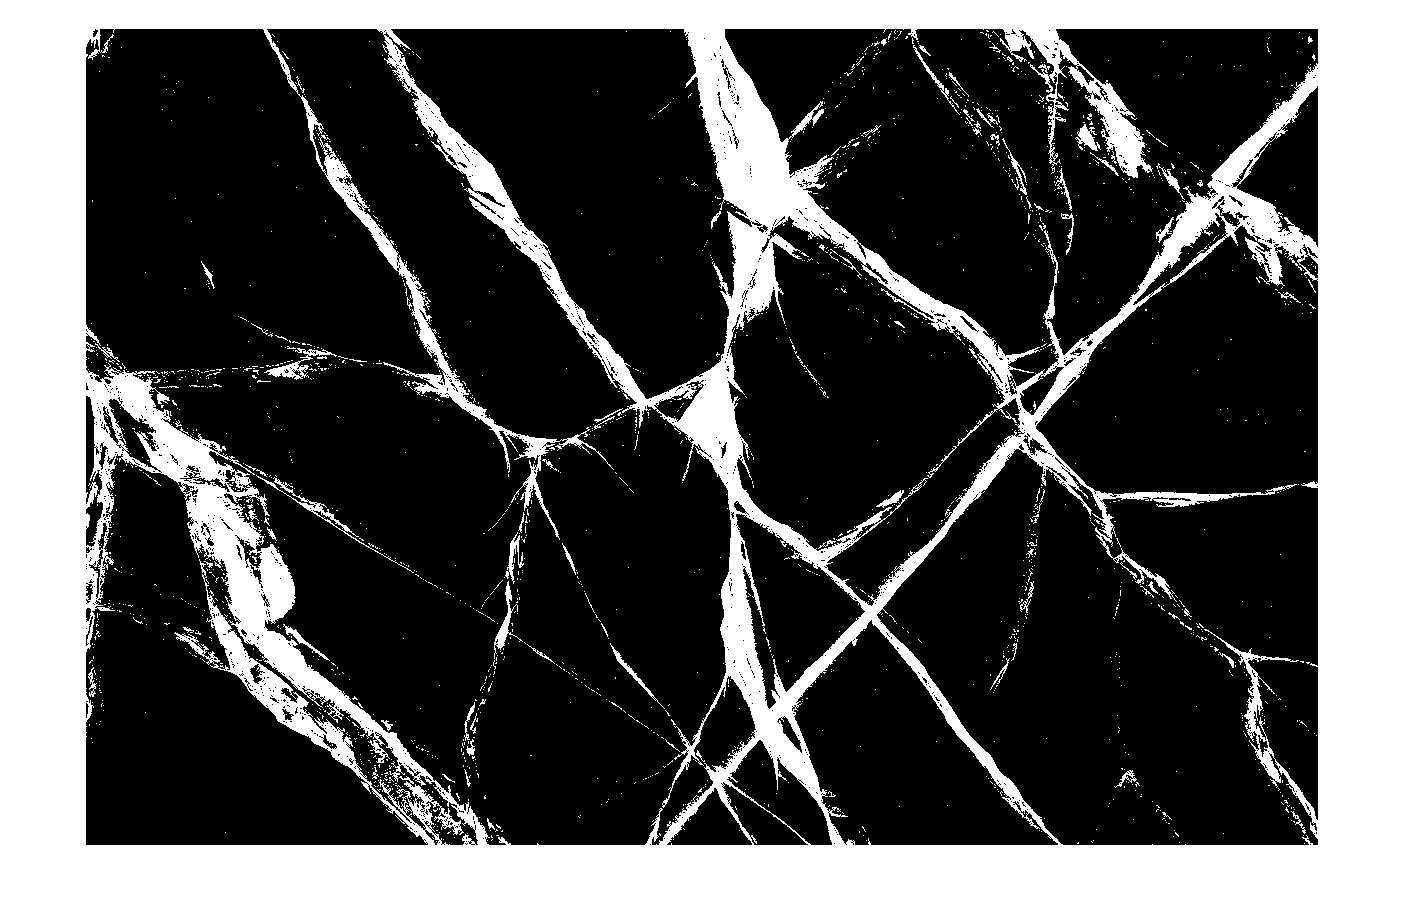
\includegraphics[width=\textwidth]{litreview/imageprocessing/nonlinear/morphology/ice_binary}
        \caption{Binarized image}
        \label{fig:ice_binary}
    \end{subfigure}
    \begin{subfigure}[b]{0.49\textwidth}
        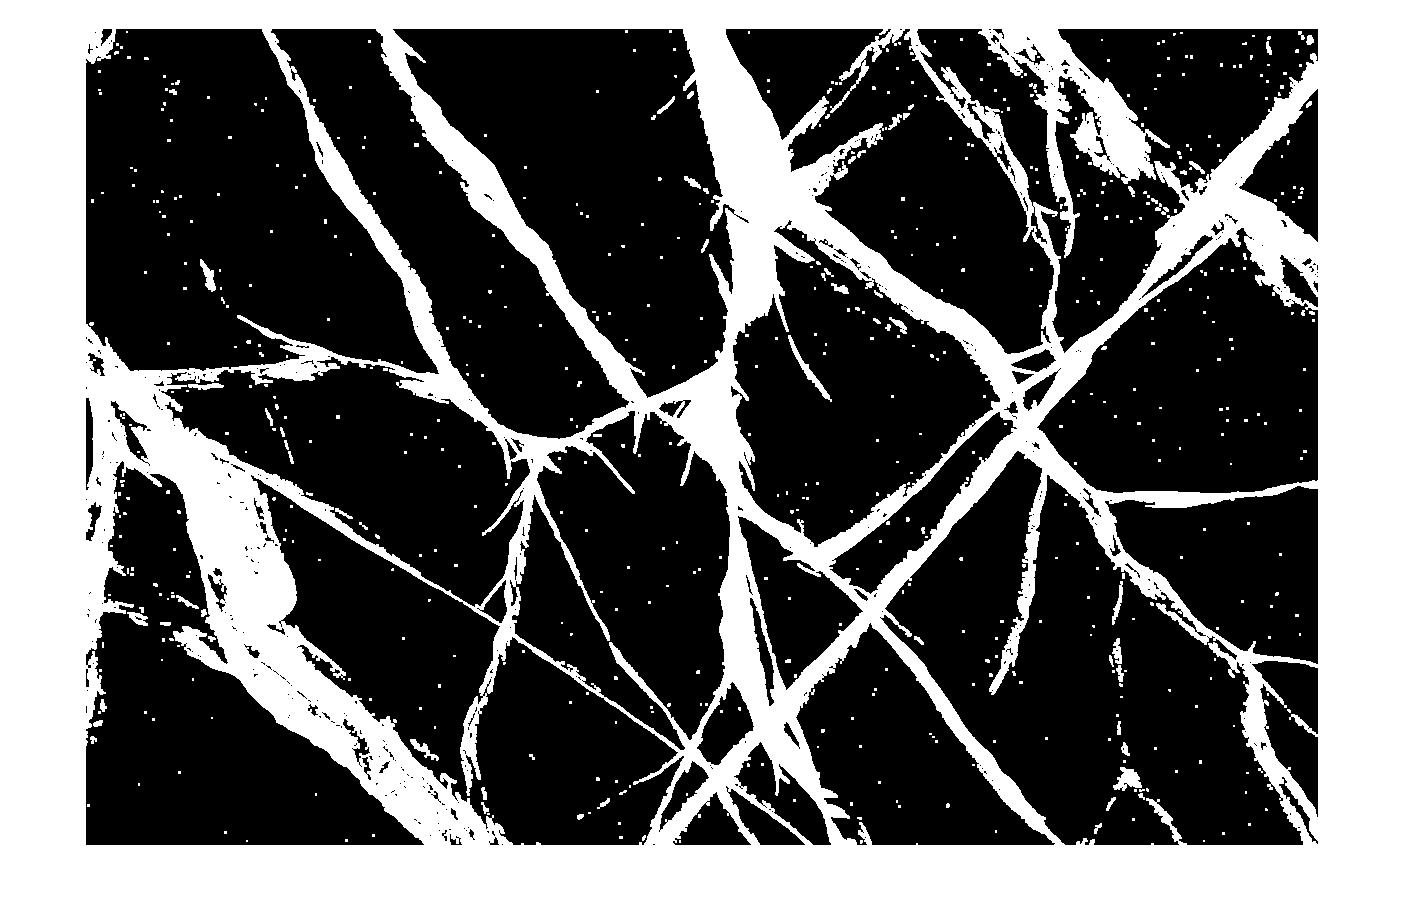
\includegraphics[width=\textwidth]{litreview/imageprocessing/nonlinear/morphology/ice_dilate}
        \caption{Dilation}
        \label{fig:ice_dilation}
    \end{subfigure}
    \begin{subfigure}[b]{0.49\textwidth}
        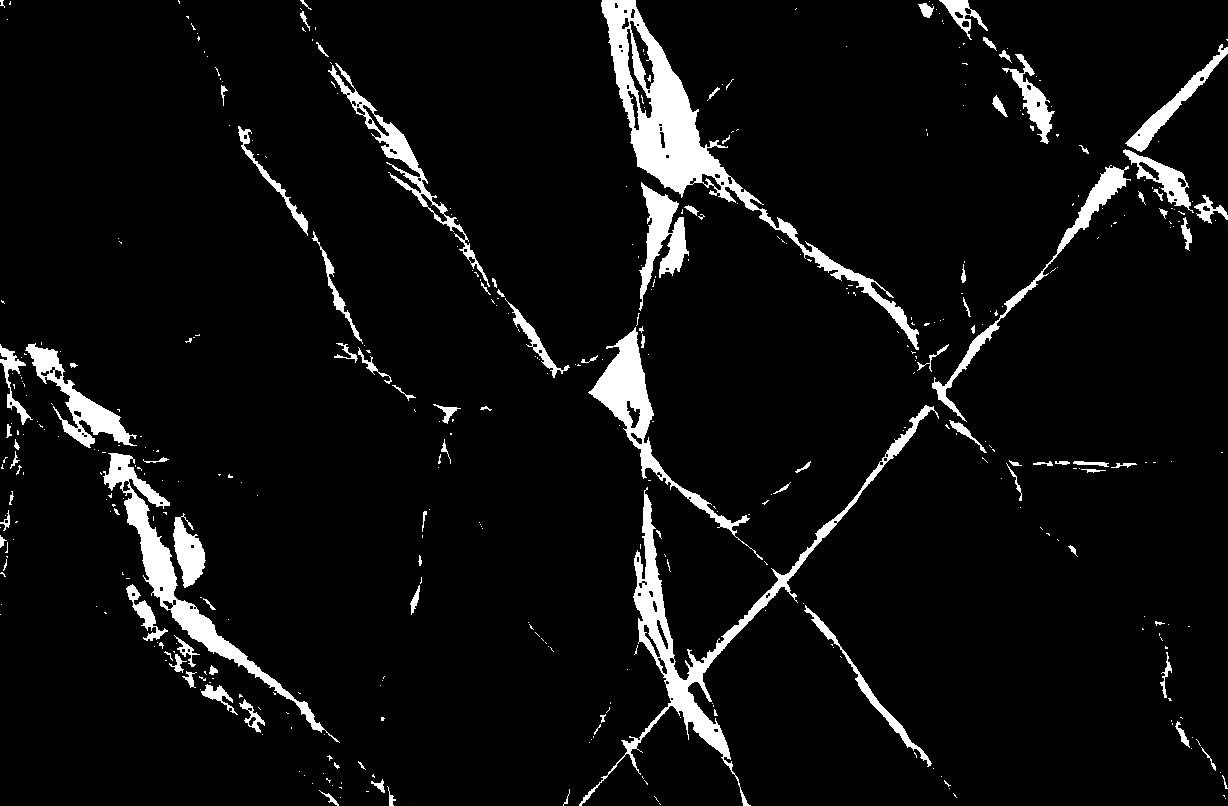
\includegraphics[width=\textwidth]{litreview/imageprocessing/nonlinear/morphology/ice_erode}
        \caption{Erosion}
        \label{fig:ice_erosion}
    \end{subfigure}
    \begin{subfigure}[b]{0.49\textwidth}
        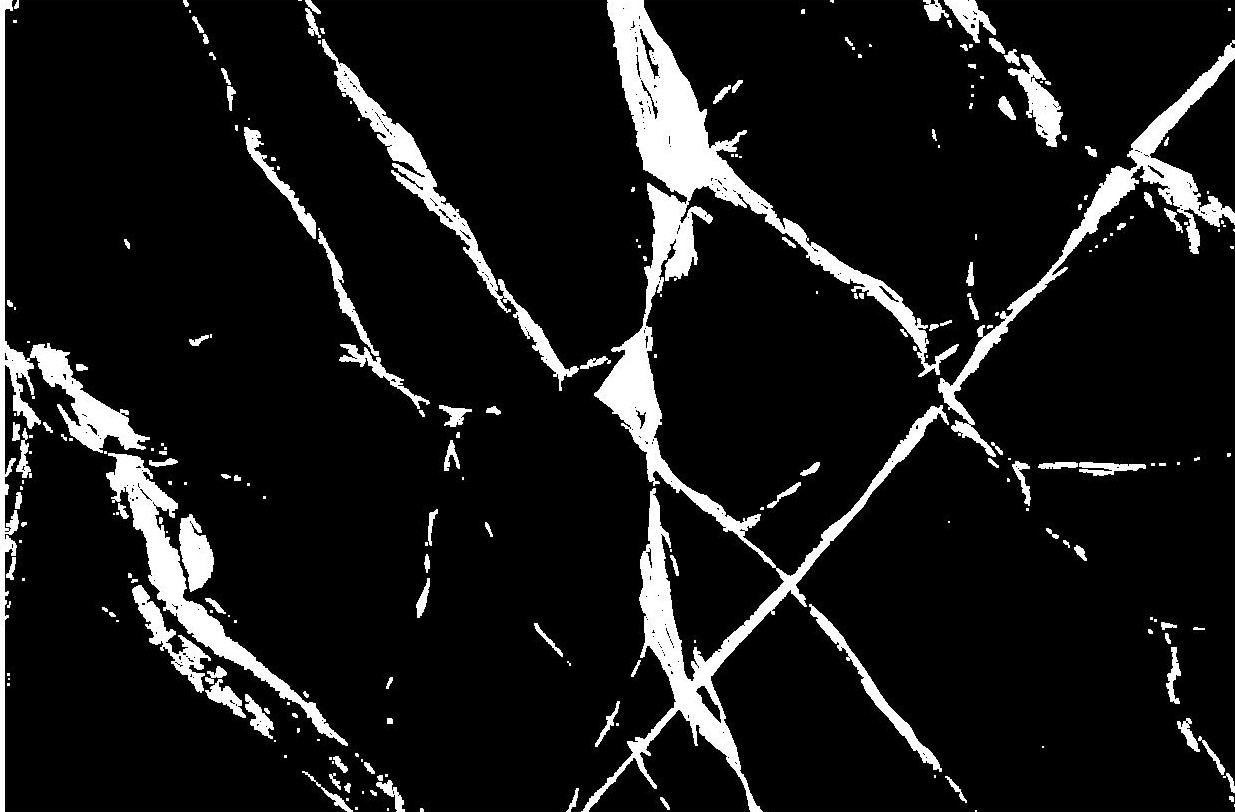
\includegraphics[width=\textwidth]{litreview/imageprocessing/nonlinear/morphology/ice_open}
        \caption{Opening}
        \label{fig:ice_open}
    \end{subfigure} 
    \begin{subfigure}[b]{0.49\textwidth}
        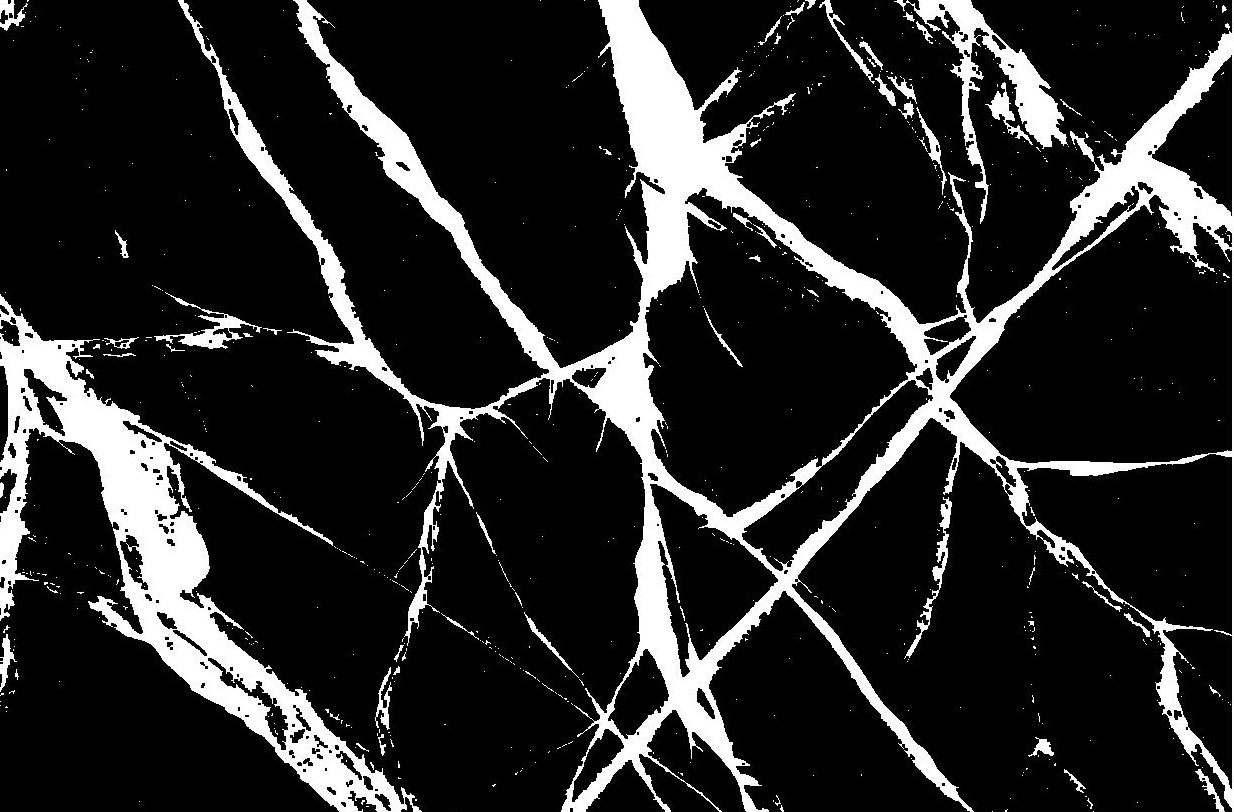
\includegraphics[width=\textwidth]{litreview/imageprocessing/nonlinear/morphology/ice_close}
        \caption{Closing}
        \label{fig:ice_close}
    \end{subfigure} 
    \captionsetup{format = hang}
    \caption{Fundamental morphological  operations performed on a binary image using a 9x9 square structuring element.}
    \label{fig:morphology}
  \end{figure}


